
%% bare_conf.tex
%% V1.3
%% 2007/01/11
%% by Michael Shell
%% See:
%% http://www.michaelshell.org/
%% for current contact information.
%%
%% This is a skeleton file demonstrating the use of IEEEtran.cls
%% (requires IEEEtran.cls version 1.7 or later) with an IEEE conference paper.
%%
%% Support sites:
%% http://www.michaelshell.org/tex/ieeetran/
%% http://www.ctan.org/tex-archive/macros/latex/contrib/IEEEtran/
%% and
%% http://www.ieee.org/







%%*************************************************************************
%% Legal Notice:
%% This code is offered as-is without any warranty either expressed or
%% implied; without even the implied warranty of MERCHANTABILITY or
%% FITNESS FOR A PARTICULAR PURPOSE! 
%% User assumes all risk.
%% In no event shall IEEE or any contributor to this code be liable for
%% any damages or losses, including, but not limited to, incidental,
%% consequential, or any other damages, resulting from the use or misuse
%% of any information contained here.
%%
%% All comments are the opinions of their respective authors and are not
%% necessarily endorsed by the IEEE.
%%
%% This work is distributed under the LaTeX Project Public License (LPPL)
%% ( http://www.latex-project.org/ ) version 1.3, and may be freely used,
%% distributed and modified. A copy of the LPPL, version 1.3, is included
%% in the base LaTeX documentation of all distributions of LaTeX released
%% 2003/12/01 or later.
%% Retain all contribution notices and credits.
%% ** Modified files should be clearly indicated as such, including  **
%% ** renaming them and changing author support contact information. **
%%
%% File list of work: IEEEtran.cls, IEEEtran_HOWTO.pdf, bare_adv.tex,
%%                    bare_conf.tex, bare_jrnl.tex, bare_jrnl_compsoc.tex
%%*************************************************************************

% *** Authors should verify (and, if needed, correct) their LaTeX system  ***
% *** with the testflow diagnostic prior to trusting their LaTeX platform ***
% *** with production work. IEEE's font choices can trigger bugs that do  ***
% *** not appear when using other class files.                            ***
% The testflow support page is at:
% http://www.michaelshell.org/tex/testflow/



% Note that the a4paper option is mainly intended so that authors in
% countries using A4 can easily print to A4 and see how their papers will
% look in print - the typesetting of the document will not typically be
% affected with changes in paper size (but the bottom and side margins will).
% Use the testflow package mentioned above to verify correct handling of
% both paper sizes by the user's LaTeX system.
%
% Also note that the "draftcls" or "draftclsnofoot", not "draft", option
% should be used if it is desired that the figures are to be displayed in
% draft mode.
%
\documentclass[conference]{IEEEtran}
% Add the compsoc option for Computer Society conferences.
%
% If IEEEtran.cls has not been installed into the LaTeX system files,
% manually specify the path to it like:
% \documentclass[conference]{../sty/IEEEtran}





% Some very useful LaTeX packages include:
% (uncomment the ones you want to load)


% *** MISC UTILITY PACKAGES ***
%
%\usepackage{ifpdf}
% Heiko Oberdiek's ifpdf.sty is very useful if you need conditional
% compilation based on whether the output is pdf or dvi.
% usage:
% \ifpdf
%   % pdf code
% \else
%   % dvi code
% \fi
% The latest version of ifpdf.sty can be obtained from:
% http://www.ctan.org/tex-archive/macros/latex/contrib/oberdiek/
% Also, note that IEEEtran.cls V1.7 and later provides a builtin
% \ifCLASSINFOpdf conditional that works the same way.
% When switching from latex to pdflatex and vice-versa, the compiler may
% have to be run twice to clear warning/error messages.

\usepackage{graphicx}

\usepackage{subfigure}
\usepackage[center]{caption}
\usepackage{url} 

% *** CITATION PACKAGES ***
%
%\usepackage{cite}
% cite.sty was written by Donald Arseneau
% V1.6 and later of IEEEtran pre-defines the format of the cite.sty package
% \cite{} output to follow that of IEEE. Loading the cite package will
% result in citation numbers being automatically sorted and properly
% "compressed/ranged". e.g., [1], [9], [2], [7], [5], [6] without using
% cite.sty will become [1], [2], [5]--[7], [9] using cite.sty. cite.sty's
% \cite will automatically add leading space, if needed. Use cite.sty's
% noadjust option (cite.sty V3.8 and later) if you want to turn this off.
% cite.sty is already installed on most LaTeX systems. Be sure and use
% version 4.0 (2003-05-27) and later if using hyperref.sty. cite.sty does
% not currently provide for hyperlinked citations.
% The latest version can be obtained at:
% http://www.ctan.org/tex-archive/macros/latex/contrib/cite/
% The documentation is contained in the cite.sty file itself.






% *** GRAPHICS RELATED PACKAGES ***
%
\ifCLASSINFOpdf
  % \usepackage[pdftex]{graphicx}
  % declare the path(s) where your graphic files are
  % \graphicspath{{../pdf/}{../jpeg/}}
  % and their extensions so you won't have to specify these with
  % every instance of \includegraphics
  % \DeclareGraphicsExtensions{.pdf,.jpeg,.png}
\else
  % or other class option (dvipsone, dvipdf, if not using dvips). graphicx
  % will default to the driver specified in the system graphics.cfg if no
  % driver is specified.
  % \usepackage[dvips]{graphicx}
  % declare the path(s) where your graphic files are
  % \graphicspath{{../eps/}}
  % and their extensions so you won't have to specify these with
  % every instance of \includegraphics
  % \DeclareGraphicsExtensions{.eps}
\fi
% graphicx was written by David Carlisle and Sebastian Rahtz. It is
% required if you want graphics, photos, etc. graphicx.sty is already
% installed on most LaTeX systems. The latest version and documentation can
% be obtained at: 
% http://www.ctan.org/tex-archive/macros/latex/required/graphics/
% Another good source of documentation is "Using Imported Graphics in
% LaTeX2e" by Keith Reckdahl which can be found as epslatex.ps or
% epslatex.pdf at: http://www.ctan.org/tex-archive/info/
%
% latex, and pdflatex in dvi mode, support graphics in encapsulated
% postscript (.eps) format. pdflatex in pdf mode supports graphics
% in .pdf, .jpeg, .png and .mps (metapost) formats. Users should ensure
% that all non-photo figures use a vector format (.eps, .pdf, .mps) and
% not a bitmapped formats (.jpeg, .png). IEEE frowns on bitmapped formats
% which can result in "jaggedy"/blurry rendering of lines and letters as
% well as large increases in file sizes.
%
% You can find documentation about the pdfTeX application at:
% http://www.tug.org/applications/pdftex





% *** MATH PACKAGES ***
%
%\usepackage[cmex10]{amsmath}
% A popular package from the American Mathematical Society that provides
% many useful and powerful commands for dealing with mathematics. If using
% it, be sure to load this package with the cmex10 option to ensure that
% only type 1 fonts will utilized at all point sizes. Without this option,
% it is possible that some math symbols, particularly those within
% footnotes, will be rendered in bitmap form which will result in a
% document that can not be IEEE Xplore compliant!
%
% Also, note that the amsmath package sets \interdisplaylinepenalty to 10000
% thus preventing page breaks from occurring within multiline equations. Use:
%\interdisplaylinepenalty=2500
% after loading amsmath to restore such page breaks as IEEEtran.cls normally
% does. amsmath.sty is already installed on most LaTeX systems. The latest
% version and documentation can be obtained at:
% http://www.ctan.org/tex-archive/macros/latex/required/amslatex/math/





% *** SPECIALIZED LIST PACKAGES ***
%
%\usepackage{algorithmic}
% algorithmic.sty was written by Peter Williams and Rogerio Brito.
% This package provides an algorithmic environment fo describing algorithms.
% You can use the algorithmic environment in-text or within a figure
% environment to provide for a floating algorithm. Do NOT use the algorithm
% floating environment provided by algorithm.sty (by the same authors) or
% algorithm2e.sty (by Christophe Fiorio) as IEEE does not use dedicated
% algorithm float types and packages that provide these will not provide
% correct IEEE style captions. The latest version and documentation of
% algorithmic.sty can be obtained at:
% http://www.ctan.org/tex-archive/macros/latex/contrib/algorithms/
% There is also a support site at:
% http://algorithms.berlios.de/index.html
% Also of interest may be the (relatively newer and more customizable)
% algorithmicx.sty package by Szasz Janos:
% http://www.ctan.org/tex-archive/macros/latex/contrib/algorithmicx/




% *** ALIGNMENT PACKAGES ***
%
%\usepackage{array}
% Frank Mittelbach's and David Carlisle's array.sty patches and improves
% the standard LaTeX2e array and tabular environments to provide better
% appearance and additional user controls. As the default LaTeX2e table
% generation code is lacking to the point of almost being broken with
% respect to the quality of the end results, all users are strongly
% advised to use an enhanced (at the very least that provided by array.sty)
% set of table tools. array.sty is already installed on most systems. The
% latest version and documentation can be obtained at:
% http://www.ctan.org/tex-archive/macros/latex/required/tools/


%\usepackage{mdwmath}
%\usepackage{mdwtab}
% Also highly recommended is Mark Wooding's extremely powerful MDW tools,
% especially mdwmath.sty and mdwtab.sty which are used to format equations
% and tables, respectively. The MDWtools set is already installed on most
% LaTeX systems. The lastest version and documentation is available at:
% http://www.ctan.org/tex-archive/macros/latex/contrib/mdwtools/


% IEEEtran contains the IEEEeqnarray family of commands that can be used to
% generate multiline equations as well as matrices, tables, etc., of high
% quality.


%\usepackage{eqparbox}
% Also of notable interest is Scott Pakin's eqparbox package for creating
% (automatically sized) equal width boxes - aka "natural width parboxes".
% Available at:
% http://www.ctan.org/tex-archive/macros/latex/contrib/eqparbox/





% *** SUBFIGURE PACKAGES ***
%\usepackage[tight,footnotesize]{subfigure}
% subfigure.sty was written by Steven Douglas Cochran. This package makes it
% easy to put subfigures in your figures. e.g., "Figure 1a and 1b". For IEEE
% work, it is a good idea to load it with the tight package option to reduce
% the amount of white space around the subfigures. subfigure.sty is already
% installed on most LaTeX systems. The latest version and documentation can
% be obtained at:
% http://www.ctan.org/tex-archive/obsolete/macros/latex/contrib/subfigure/
% subfigure.sty has been superceeded by subfig.sty.



%\usepackage[caption=false]{caption}
%\usepackage[font=footnotesize]{subfig}
% subfig.sty, also written by Steven Douglas Cochran, is the modern
% replacement for subfigure.sty. However, subfig.sty requires and
% automatically loads Axel Sommerfeldt's caption.sty which will override
% IEEEtran.cls handling of captions and this will result in nonIEEE style
% figure/table captions. To prevent this problem, be sure and preload
% caption.sty with its "caption=false" package option. This is will preserve
% IEEEtran.cls handing of captions. Version 1.3 (2005/06/28) and later 
% (recommended due to many improvements over 1.2) of subfig.sty supports
% the caption=false option directly:
%\usepackage[caption=false,font=footnotesize]{subfig}
%
% The latest version and documentation can be obtained at:
% http://www.ctan.org/tex-archive/macros/latex/contrib/subfig/
% The latest version and documentation of caption.sty can be obtained at:
% http://www.ctan.org/tex-archive/macros/latex/contrib/caption/




% *** FLOAT PACKAGES ***
%
%\usepackage{fixltx2e}
% fixltx2e, the successor to the earlier fix2col.sty, was written by
% Frank Mittelbach and David Carlisle. This package corrects a few problems
% in the LaTeX2e kernel, the most notable of which is that in current
% LaTeX2e releases, the ordering of single and double column floats is not
% guaranteed to be preserved. Thus, an unpatched LaTeX2e can allow a
% single column figure to be placed prior to an earlier double column
% figure. The latest version and documentation can be found at:
% http://www.ctan.org/tex-archive/macros/latex/base/



%\usepackage{stfloats}
% stfloats.sty was written by Sigitas Tolusis. This package gives LaTeX2e
% the ability to do double column floats at the bottom of the page as well
% as the top. (e.g., "\begin{figure*}[!b]" is not normally possible in
% LaTeX2e). It also provides a command:
%\fnbelowfloat
% to enable the placement of footnotes below bottom floats (the standard
% LaTeX2e kernel puts them above bottom floats). This is an invasive package
% which rewrites many portions of the LaTeX2e float routines. It may not work
% with other packages that modify the LaTeX2e float routines. The latest
% version and documentation can be obtained at:
% http://www.ctan.org/tex-archive/macros/latex/contrib/sttools/
% Documentation is contained in the stfloats.sty comments as well as in the
% presfull.pdf file. Do not use the stfloats baselinefloat ability as IEEE
% does not allow \baselineskip to stretch. Authors submitting work to the
% IEEE should note that IEEE rarely uses double column equations and
% that authors should try to avoid such use. Do not be tempted to use the
% cuted.sty or midfloat.sty packages (also by Sigitas Tolusis) as IEEE does
% not format its papers in such ways.





% *** PDF, URL AND HYPERLINK PACKAGES ***
%
%\usepackage{url}
% url.sty was written by Donald Arseneau. It provides better support for
% handling and breaking URLs. url.sty is already installed on most LaTeX
% systems. The latest version can be obtained at:
% http://www.ctan.org/tex-archive/macros/latex/contrib/misc/
% Read the url.sty source comments for usage information. Basically,
% \url{my_url_here}.





% *** Do not adjust lengths that control margins, column widths, etc. ***
% *** Do not use packages that alter fonts (such as pslatex).         ***
% There should be no need to do such things with IEEEtran.cls V1.6 and later.
% (Unless specifically asked to do so by the journal or conference you plan
% to submit to, of course. )


% correct bad hyphenation here
\hyphenation{op-tical net-works semi-conduc-tor}

\usepackage{color}

\begin{document}
%
% paper title
% can use linebreaks \\ within to get better formatting as desired
\title{A Google Android based communication interface with Smart Homes sensing devices}


% author names and affiliations
% use a multiple column layout for up to three different
% affiliations
\author{\IEEEauthorblockN{Dimitrios Archontis, Spyros Kehagias, Vasilis Maglogiannis, Nikos Makris,\\ Virgilios Passas, Ilias Syrigos, Kostas Hounos and Lefteri H. Tsoukala}
\IEEEauthorblockA{Dept. of Electrical and Computer Engineering\\
University of Thessaly, 
Volos, Greece\\
Email: \{arhontis, spkehagi, vamaglog, nimakris, vipassas, ilsyrigo, hounos\}@uth.gr  $|$ tsoukala@ecn.purdue.edu}

%\and


%\IEEEauthorblockN{Lefteri H. Tsoukala}
%\IEEEauthorblockA{Dept. of Electrical and\\Computer Engineering\\
%University of Thessaly \\
%Volos, Greece\\
%Email: tsoukala@ecn.purdue.edu}
}

% conference papers do not typically use \thanks and this command
% is locked out in conference mode. If really needed, such as for
% the acknowledgment of grants, issue a \IEEEoverridecommandlockouts
% after \documentclass

% for over three affiliations, or if they all won't fit within the width
% of the page, use this alternative format:
% 
%\author{\IEEEauthorblockN{Michael Shell\IEEEauthorrefmark{1},
%Homer Simpson\IEEEauthorrefmark{2},
%James Kirk\IEEEauthorrefmark{3}, 
%Montgomery Scott\IEEEauthorrefmark{3} and
%Eldon Tyrell\IEEEauthorrefmark{4}}
%\IEEEauthorblockA{\IEEEauthorrefmark{1}School of Electrical and Computer Engineering\\
%Georgia Institute of Technology,
%Atlanta, Georgia 30332--0250\\ Email: see http://www.michaelshell.org/contact.html}
%\IEEEauthorblockA{\IEEEauthorrefmark{2}Twentieth Century Fox, Springfield, USA\\
%Email: homer@thesimpsons.com}
%\IEEEauthorblockA{\IEEEauthorrefmark{3}Starfleet Academy, San Francisco, California 96678-2391\\
%Telephone: (800) 555--1212, Fax: (888) 555--1212}
%\IEEEauthorblockA{\IEEEauthorrefmark{4}Tyrell Inc., 123 Replicant Street, Los Angeles, California 90210--4321}}




% use for special paper notices
%\IEEEspecialpapernotice{(Invited Paper)}




% make the title area
\maketitle


\begin{abstract}
%\boldmath
The rapid evolution of Wireless Sensor Networks (WSN) lately, has been the stimulus for the establishment of Smart Houses. 
A Smart House (SH) is a house that has highly advanced automatic systems for lighting, temperature control, multi-media, security, window and door operations, and many other functions. 
Wireless technologies that are exploited in a SH installation are usually the WiFi and ZigBee protocol, due to the freedom of operating devices in the unlicensed band of 2.4 GHz. 
In this paper, we utilize the WSN devices developed by the NITLab laboratory in University of Thessaly and a Plugwise “Home Basic” kit, and design and implement an Android application able to retrieve data and measurements from these sensors, and represent them to the end user providing a user-friendly GUI.


\end{abstract}
% IEEEtran.cls defaults to using nonbold math in the Abstract.
% This preserves the distinction between vectors and scalars. However,
% if the conference you are submitting to favors bold math in the abstract,
% then you can use LaTeX's standard command \boldmath at the very start
% of the abstract to achieve this. Many IEEE journals/conferences frown on
% math in the abstract anyway.

% no keywords




% For peer review papers, you can put extra information on the cover
% page as needed:
% \ifCLASSOPTIONpeerreview
% \begin{center} \bfseries EDICS Category: 3-BBND \end{center}
% \fi
%
% For peerreview papers, this IEEEtran command inserts a page break and
% creates the second title. It will be ignored for other modes.
\IEEEpeerreviewmaketitle



\section{Introduction}
% no \IEEEPARstart
Over the past few years, the idea of Smart Homes (SHs) has become more and more attractive.
SH connect all the devices and appliances in an ordinary home so they can communicate with each other and usually with the owner. 
Anything in a home that uses electricity can be put on the home network and at one’s command. 
In the case that interaction with an SH user is available, this comes usually with several interfaces; whether a command is given by voice, remote control or computer, the home reacts. 
So far, almost all of the developed applications relate to lighting, home security, home theater and entertainment and thermostat regulation \cite{howshswork}.


Therefore, SHs are homes which utilize information appliances and a home-based network to connect household appliances to each other and to the outside Internet world.
Using sensors mounted on devices and various coordinating protocols, SH try to enhance urban living by automating ordinary life. 

SH technology first allowed compatible products to talk to each other over the already existing electrical wires of a home. 
A key technology that still utilizes such interfaces is the Power Line Communication (PLC) protocols, developed by several technology vendors.
All the appliances and devices are receivers, and the means of controlling the system, such as remote controls or keypads, are transmitters. 

Instead of going through the power lines, some systems use radio waves to communicate, which is also how WiFi and cell phone signals operate. 
However, home automation networks don't need all the features of a WiFi network because automation commands are short messages. 
The use of the unlicensed bands of 2.4GHz, has been a strong motivation for the design and development of several new protocols, specially designed for satisfying the needs of wireless communication in a SH.

Wireless networking has developed rapidly in the last years towards this direction and has contributed a great deal to this field. 
An applied technology of wireless networking is the WiFi based on the IEEE 802.11 standards.
The obvious advantage of wireless transmission is a significant reduction and simplification in wiring and harness. 
Many communication technologies, such as IrDA, Bluetooth and ZigBee, GSM/GPRS (General Packet Radio Service), etc., have been developed for different situations. 
Nowadays, a kind of real time systems in which multiple sensors connected simultaneously to one gateway unit become necessary, and they are transformed into wireless sensor networks (WSNs).

A real life application of WSNs are the SHs \cite{paper}.  
In such a case, a WSN consists of spatially distributed autonomous sensors to monitor physical or environmental conditions, such as temperature, sound, pressure, etc. and to cooperatively pass their data through the network to a main location \cite{wikiwsn}.
Usually, a server there aggregates and processes the data, and using sophisticated techniques may schedule the operation of many SH appliances, in the most efficient way.

In the following sections we give a brief overview of the most common wireless technologies that are used in a SH system. 
The common point between them is the band they transmit (usually they make use of the unlicensed bands), and their extended use worldwide.
The most common are 
\begin{itemize}

  \item The WiFi protocol
  \item The ZigBee protcol


\end{itemize}




\subsection{The WiFi protocol}

The radios used for WiFi communication are very similar to the radios used for walkie-talkies, cell phones and other devices. 
They can transmit and receive radio waves, and they can convert 1s and 0s into radio waves and convert the radio waves back into 1s and 0s. 

But WiFi radios have a few notable differences from other radios. 
They transmit at frequencies of 2.4 GHz (or 5 GHz). 
This frequency is considerably higher than the frequencies used for cell phones, walkie-talkies and televisions. 
The higher frequency allows the signal to carry more data.  
This frequency also belongs to what are called “unlicensed radio frequency bands”. 
These are used by anyone who wants to use them, without fee.
They use 802.11 networking standards, which come in several standards. 
The main standards transmitting at unlicensed frequency bands are 802.11b and 802.11g. 


\begin{itemize}

  \item 
802.11b is the slowest and least expensive standard. 
For a while, its cost made it popular, but now it's becoming less common as faster standards become less expensive. 
802.11b transmits in the 2.4 GHz frequency band of the radio spectrum. 
It can handle up to 11 megabits of data per second, and it uses complementary code keying (CCK) modulation to improve speeds.
  \item 
802.11g transmits at 2.4 GHz like 802.11b, but it's a lot faster -- it can handle up to 54 megabits of data per second. 
802.11g is faster because it uses the same OFDM coding as 802.11a.


\end{itemize}

Other protocols/standards operating in different frequency bands include 802.11a, 802.11n and 802.11ac \cite{howwifiworks}.


\subsection{The ZigBee protocol}

ZigBee is a low-cost, low-power, wireless mesh network standard. 
The low cost allows the technology to be widely deployed in wireless control and monitoring applications. 
Low power-usage allows longer life with smaller batteries. 
Mesh networking provides high reliability and more extensive range. 
ZigBee chip vendors typically sell integrated radios and microcontrollers with between 60 KB and 256 KB flash memory.
ZigBee operates in the industrial, scientific and medical (ISM) radio bands; 868 MHz in Europe, 915 MHz in the USA and Australia and 2.4 GHz in most jurisdictions worldwide. 
Data transmission rates vary from 20 kilobits/second in the 868 MHz frequency band to 250 kilobits/second in the 2.4 GHz frequency band \cite{wikiwsn}.
The ZigBee network layer natively supports both star and tree typical networks, and generic mesh networks.
 Every network must have one coordinator device, tasked with its creation, the control of its parameters and basic maintenance. 
Within star networks, the coordinator must be the central node.
 Both trees and meshes allows the use of ZigBee routers to extend communication at the network level.

\begin{figure}[!t]
\centering
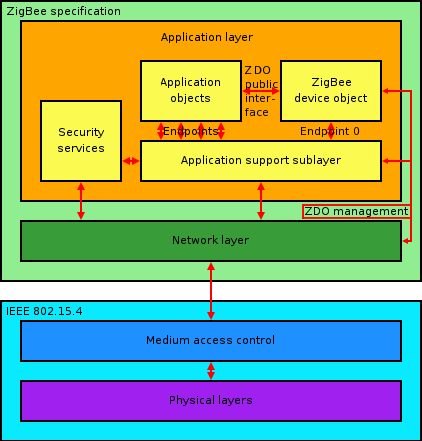
\includegraphics[width=2.5in]{images/ZigBee_protocol_stack.png}
 %where an .eps filename suffix will be assumed under latex, 
 %and a .pdf suffix will be assumed for pdflatex; or what has been declared
% via \DeclareGraphicsExtensions.
\caption{The ZigBee protocol stack}
\label{zigbee}
\end{figure}


ZigBee builds upon the physical layer and media access control defined in IEEE standard 802.15.4 (2003 version) for low-rate WPANs. 
The specification goes on to complete the standard by adding four main components: network layer, application layer, ZigBee device objects (ZDOs) and manufacturer-defined application objects which allow for customization and favor total integration.
Besides adding two high-level network layers to the underlying structure, the most significant improvement is the introduction of ZDOs.
 These are responsible for a number of tasks, which include keeping of device roles, management of requests to join a network, device discovery and security.

ZigBee is not intended to support powerline networking but to interface with it at least for smart metering and smart appliance purposes such as the ones we find in SHs.
Because ZigBee nodes can go from sleep to active mode in 30 ms or less, the latency can be low and devices can be responsive, particularly compared to Bluetooth wake-up delays, which are typically around three seconds \cite{paper}.
Because ZigBee nodes can sleep most of the time, average power consumption can be low, resulting in long battery life. 
A Bluetooth SMART device can exchange data and disconnect in 3 ms, when advertising is pushed to maximum connect. 
This significantly enhances the experiences for HID devices \cite{zigbee}.







User - SH appliance communication may be integrated into the functionality of already popular devices such as smart phones operating under various mobile operating systems. 
We developed a Google Android application, one of the world's most popular mobile platform. 
It is open source and Google releases the code under the Apache License. 
This open source code and permissive licensing allows the software to be freely modified and distributed by device manufacturers, wireless carriers and enthusiast developers. 
Additionally, Android has a large community of developers writing applications ("apps") that extend the functionality of devices \cite{android}.
Details about the design and implementation of the system are presented in the following sections.

\section{Sensing Platforms}
For this paper, we used two different technologies, able to be incorporated in a SH, and developed the Android application for retrieving the measurements from them. 
The first platform is an experimental one, completely designed and developed by University of Thessaly. 
The second one is the well known commercial platform of PlugWise, ready for integration with already existing home appliances. 
A brief overview of the platforms is presented in the following subsections.


\begin{figure*}[!t]
\begin{center}
\centering
\subfigure[NITOS Sensing Platform]{
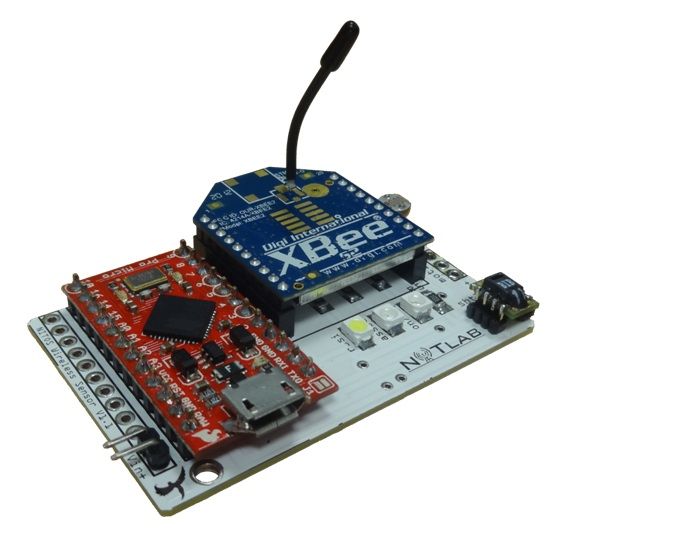
\includegraphics[width=0.8\columnwidth]{images/xbee.jpg}
\label{fig:nitoswsn}}
\hspace{0.3\columnwidth}
\subfigure[The PlugWise platform]{
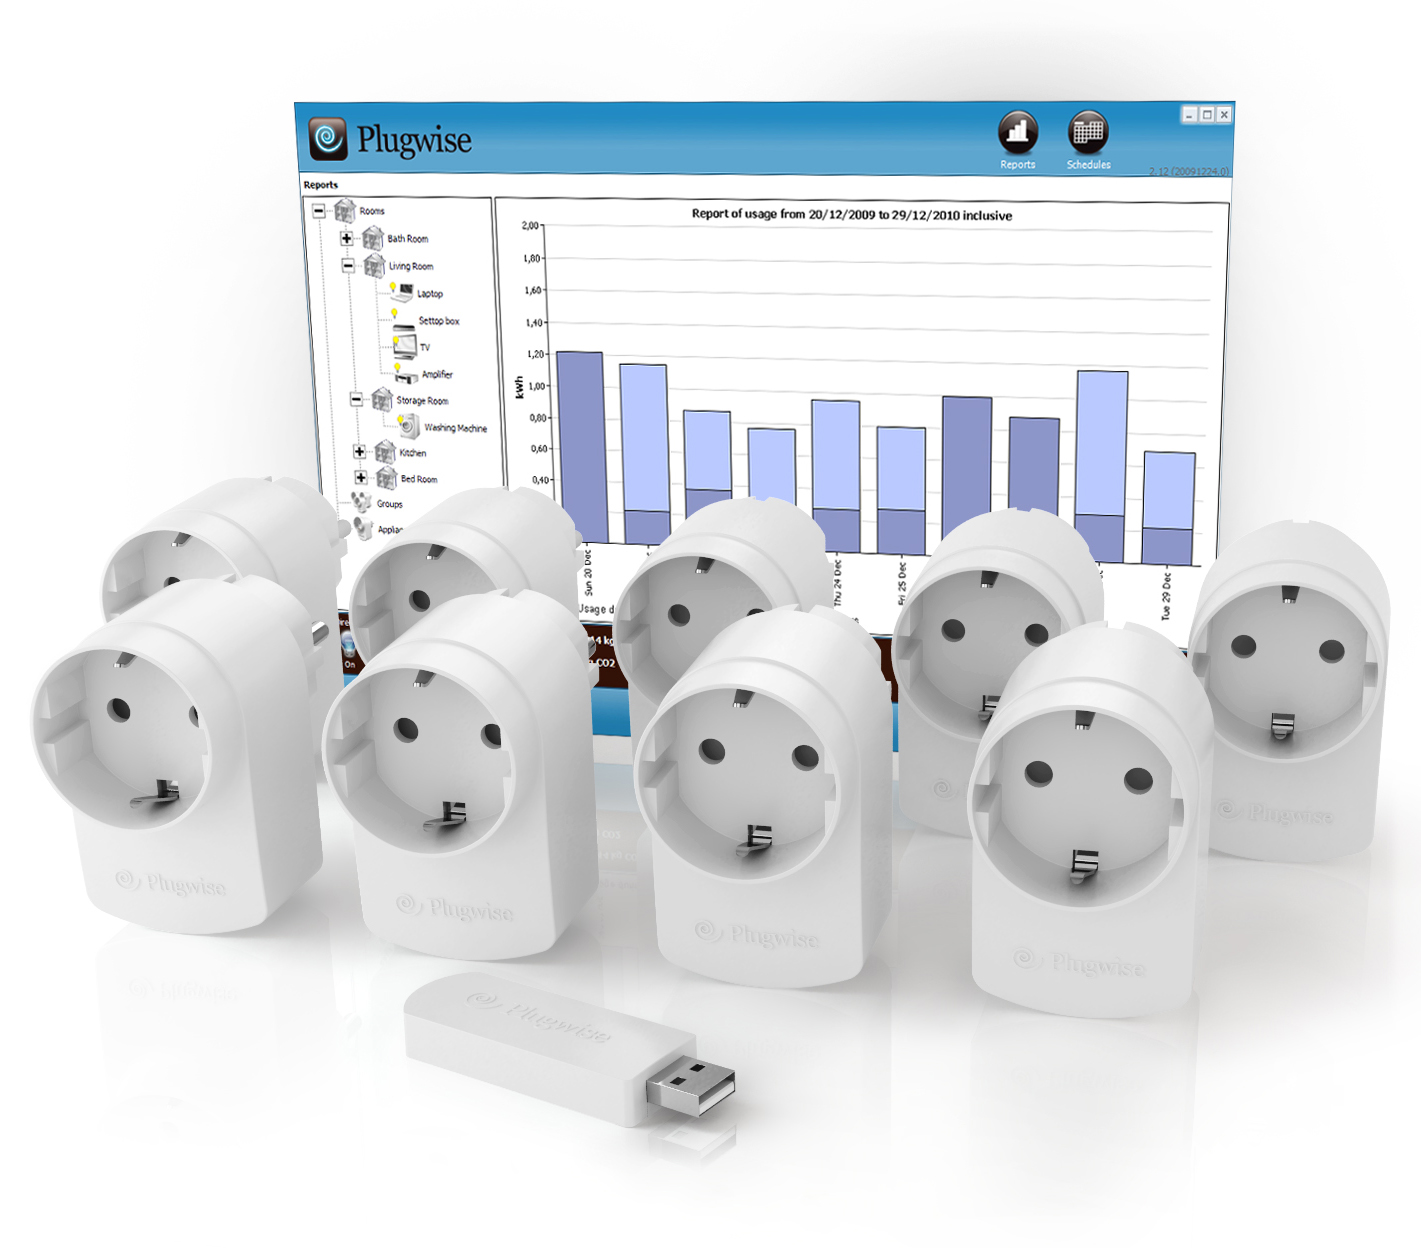
\includegraphics[width=0.8\columnwidth]{images/plugwise.jpg}
\label{fig:plugwise}}
\caption{Sensing Platforms used in our setup}

\end{center}
\vspace{-0.8cm}
\end{figure*}


\subsection{NITOS WSN platform}
To implement our solution we utilized the NITOS wireless sensor platforms. 
Towards the direction of enabling sensing based on WSN solutions, NITLab \cite{nitlab} / UTH has developed a prototype wireless sensor platform comprised of open-source and configurable modules. 
The main part of the aforementioned platform is a Pro Micro \cite{promicro} board, fabricated by Sparkfun Electronics \cite{sparkfun}, a well-known industrial company, which provides open-source hardware platforms that are fully configurable by Arduino's \cite{arduino} open-source software. 
The on-board AVR micro-controller developed by Atmel \cite{atmel}, runs at 8Mhz and coordinates the overall platform operation. 
Moreover, the platform is equipped with an Xbee \cite{xbee} radio interface that enables communication with a respective gateway. 
The Xbee module is a tiny device ideal for setting up mesh networks and has a defined rate of 250 kbps. 
This module uses the IEEE 802.15.4 stack (the basis for Zigbee \cite{zigbee-all}) and wraps it into a simple to use serial command set, allowing a very reliable and simple communication with Pro Micro's micro-controller. 


The developed platform currently features a number of sensing modules, such as air temperature and humidity, light intensity and human presence. 
Various types of sensing modules and actuators can be further integrated utilizing Arduino libraries that implement several existing communications protocols, such as I2C, LIN, SPI, TWI, USI, etc. 
Firmware can be easily uploaded through the on-board USB connection. 
In addition to this, the developed platform supports over-the-air-programming (which is visible through) achieved by a special circuit already integrated in the PCB, allowing firmware to be uploaded wirelessly. 
Apart from the pluggable Xbee module, the developed platform can be equipped with WiFi or Bluetooth radio interfaces compatible with Xbee footprint, thus enabling communication utilizing different technology standards. 
By exploiting open-source firmware, developers can define different network topologies according to their experimentation setup, while numerous aggregation schemes can be used for gathering information reducing the total communication cost. 
Finally, the developed platform is a low-cost and small-sized one that can be powered by low-voltage sources, making it ideal for extended deployment at almost any place.


\subsection{The PlugWise platform}

Our developed platform incorporates support for a “PlugWise - Home Basic kit”. 
Plugwise has developed and produced wireless systems for energy management and appliance control since 2006. 
They have released several products, mainly power consumption metering devices, which can be easily configured and integrated with existing home appliance equipment.
Such a kit is the “Home Basic Kit”, which consists of Circle+, eight Circles, the Plugwise Stick and the Source software. 
The components of the kit are depicted in Figure figure \ref{fig:plugwise}, and can be easily operated by inexperienced users. 


Plugwise Circles communicate with each other wirelessly, utilizing the 802.15.4 networking stack and a slightly altered ZigBee protocol. 
All Circles form a wireless mesh network with each other, but in case they should transmit data back to a server device, they communicate via the Circle+ plug.

Although the Plugwise platform is a commercial one, and therefore the company does not provide an official Application Interface (API) for experimentation with their products, we used a reversed-engineered python library that has become available to the community. 
However, although the API is clearly defined in this library, it is not that mature yet and extra programming effort is required. 
More details upon the problems we had to cope with when setting up our platforms concerning the software used are given in the next section.



\begin{figure*}[!t]
\begin{center}
\centering
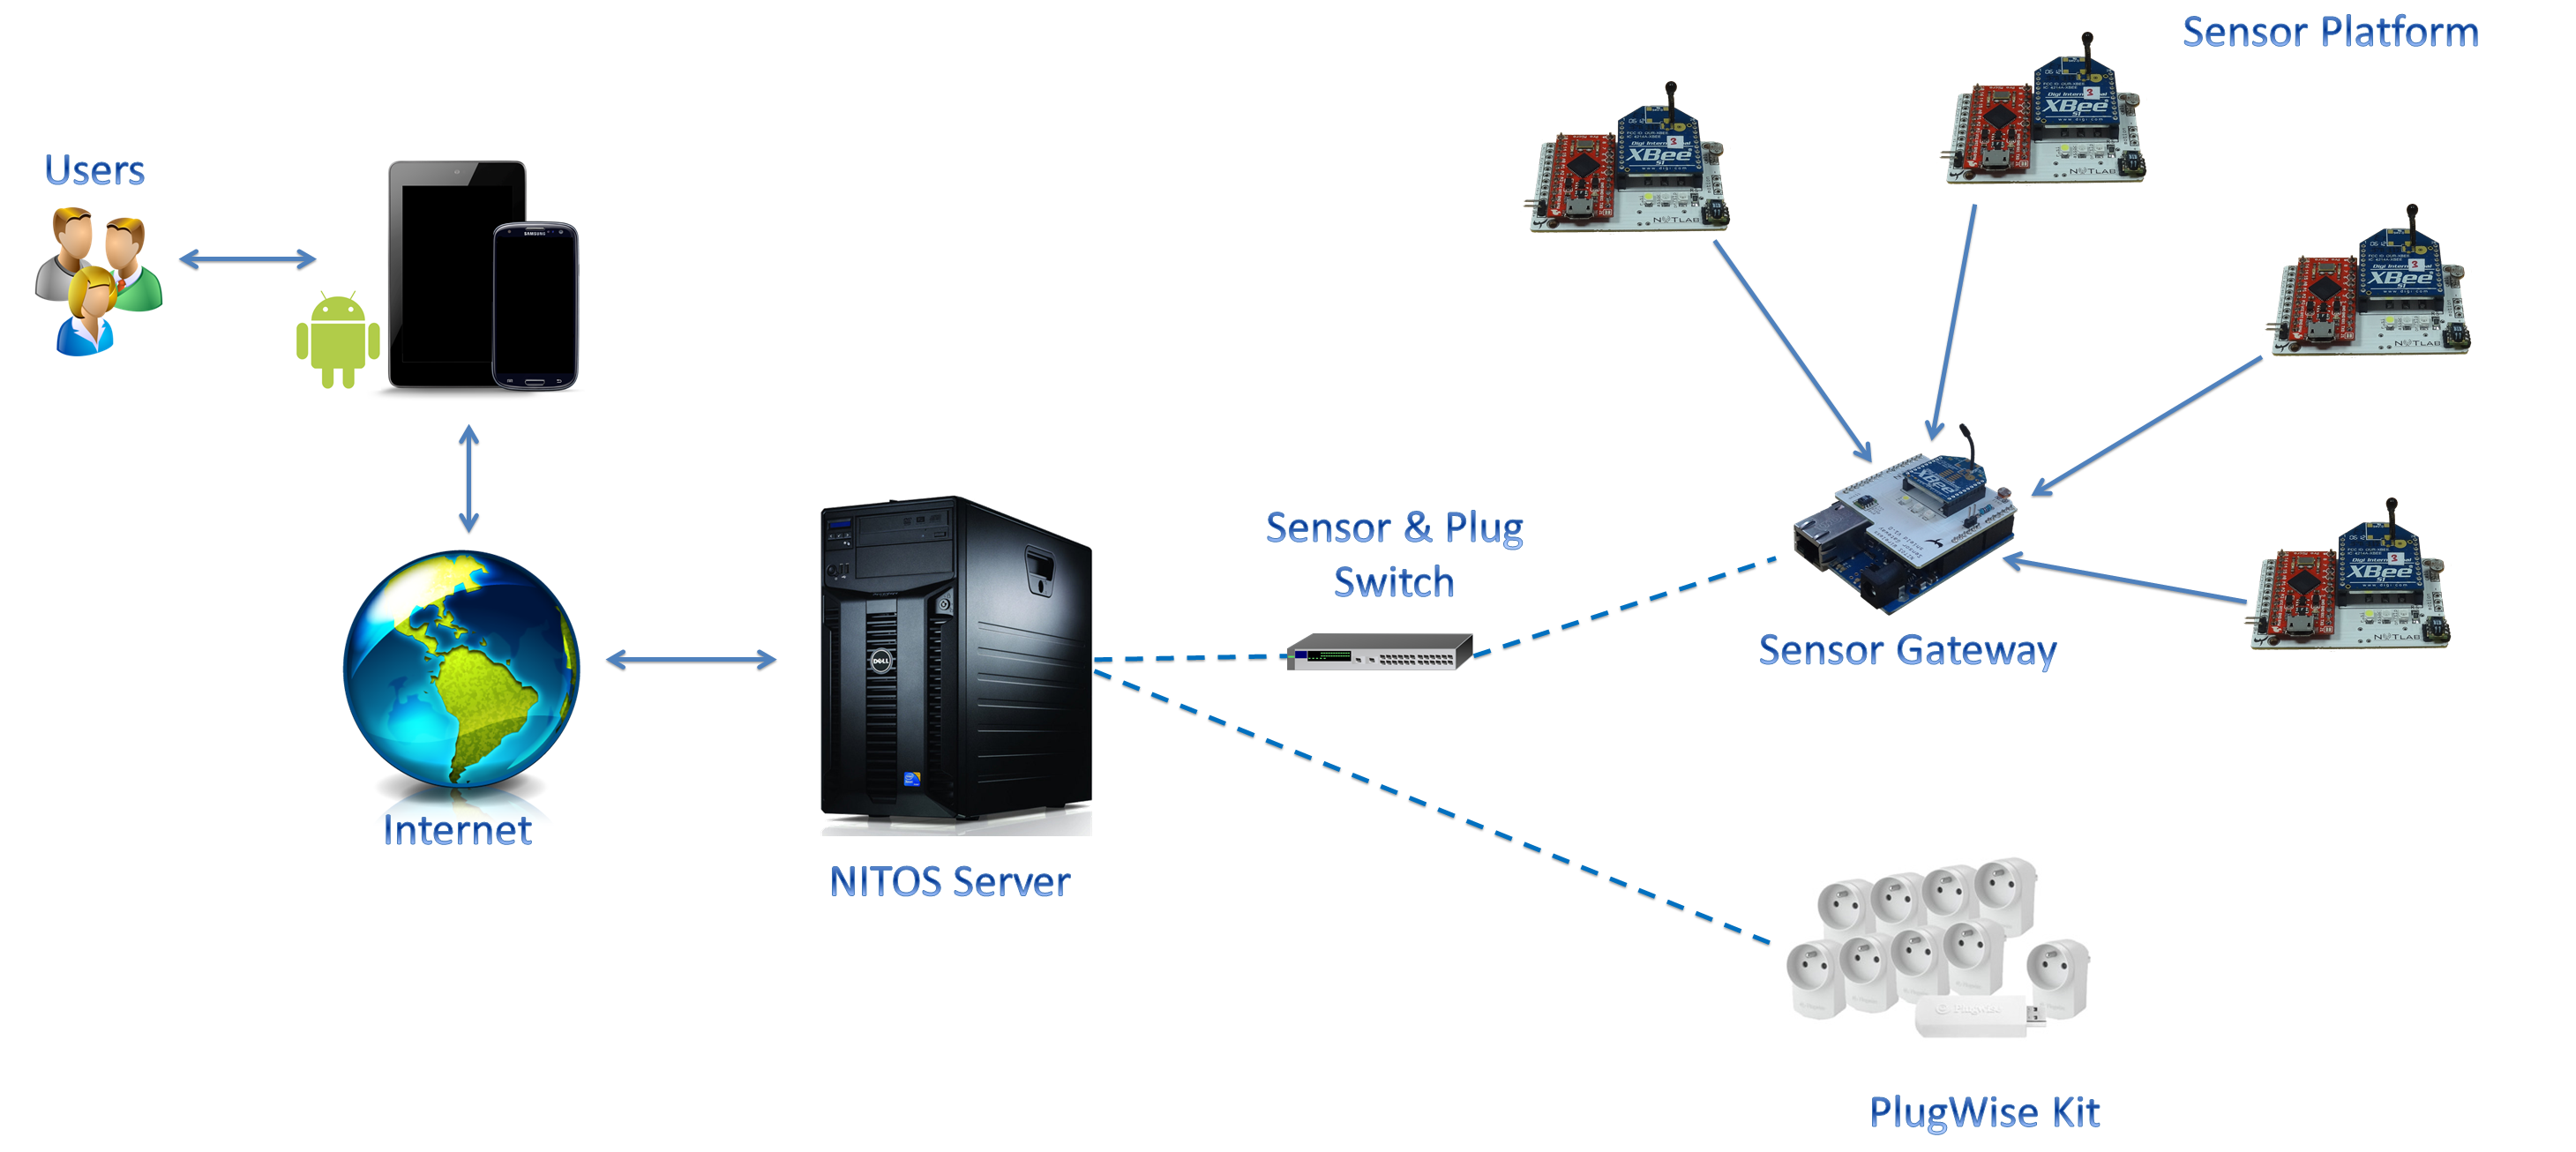
\includegraphics[scale=0.15]{images/tsoukalas_arch.png}
\caption{Our Experimental Architecture}
\label{fig:network_arch}\end{center}
\vspace{-0.8cm}
\end{figure*}




\section{Implementation Details}
In this section, we describe some implementation details, and the tools we exploited for the overall setup of the platform. We initially describe the software tools we used, and subsequently the networking setup that was required for the demonstration of our application.

\subsection{Software Tools}
Towards rendering the described hardware platform into a functional framework, we developed appropriate software in order to control wireless sensor platforms(WSPs) and the Plugwise “Home Basic Kit”. 
The four basic software components that were used are:






We exploited the capabilities of the provided source package \cite{plugwise}  so as to achieve the desired functionalities of the “Home Basic Kit”.
We are able to manage the status of the connected plugs, meaning that we have the ability  to switch them on or off. 
Moreover we can retrieve the instantaneous power consumption(in Watts) of every plug, as well as the average consumption of each plug and of the whole Kit. 

Concerning our implementation, we decided that in order for our approach to have some feasible results, we needed to write several python scripts that would operate in the backend of our system, and would actually instrument the Plugwise hardware operation. 
The operations that we needed to support are: switching on/off the PlugWise Circles, get the instantaneous power consumption and the average power consumption in Watts. 
Since the average consumption values are not supporteed by the API we used, we wrote a daemon process that wakes up periodically, and asks the device for the value of its current power consumption. 

\subsubsection{Arduino IDE}
The Arduino integrated development environment (IDE) \cite{arduino-ide} is a cross-platform application written in Java, and is derived from the IDE for the Processing programming language and the Wiring projects.
It is designed to introduce programming to artists and other newcomers unfamiliar with software development. 
It includes a code editor with features such as syntax highlighting, brace matching, and automatic indentation, and is also capable of compiling and uploading programs to the board with a single click. 
There is typically no need to edit makefiles or run programs on a command-line interface. A program or code written for Arduino is called a sketch. 
Arduino libraries are written in C or C++. 
The Arduino IDE comes with a software library called "Wiring" from the original Wiring project, which makes many common input/output operations much easier. 
Users only need define two functions to make a runnable cyclic executive program:
\begin{itemize}
\item setup():  a function run once at the start of a program that can initialize settings
\item loop()  :  a function called repeatedly until the board powers off.
\end{itemize}

We employed the Arduino IDE in order to manage the wireless sensor platforms and the gateway. 
The former`’s implemented functionality is to collect periodically the values of the existing attached sensors and send them to the gateway through the Zigbee Protocol 802.15.4. 
The gateway remains active and waits for receiving packets from WSPs.
Every incoming packet triggers another function of the gateway which sends the packet to NITOS server using the ethernet interface attached on it.  

\subsubsection{Android API - Appccelerator IDE}
Android SDK is a software development kit that enables developers to create applications for the Android platform. 
The Android SDK includes sample projects with source code, development tools, an emulator, and required libraries to build Android applications. 
Applications are written using the Java programming language and run on Dalvik, a custom virtual machine designed for embedded use which runs on top of a Linux kernel. 
Android SDK includes several API’s each one according to a specific Android OS version. 
Our application has been developed with API level 14 and it supports every Android version newer than 3.2 .
Due to our previous experience in developing Android applications using Appccelarator we chose to take advantage of the various capabilities offered by it and develop our application.  



\begin{figure*}[!t]
\begin{center}
\centering
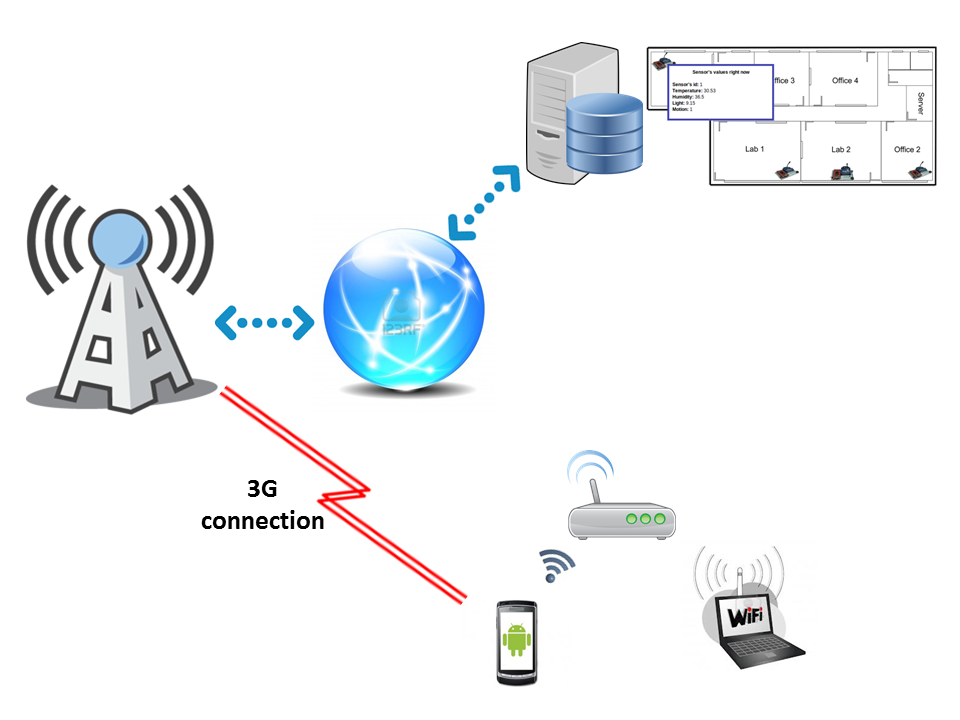
\includegraphics[scale=0.35]{images/Demo_Setup.png}
\caption{Networking setup for demonstration needs}
\label{fig:network}
\end{center}
\vspace{-0.8cm}
\end{figure*}

Appcelerator Titanium Mobile is one of several phone web based application framework solutions allowing web developers to apply existing skills to create native applications for iPhone and Android.
Instead of using the familiar JavaScript syntax, developers can also use Ajax, JQuery, HTML and CSS frameworks. 
For the evaluation of our developed application we utilized Appccelarator emulator, so as to preview and test application for possible errors.
The objective of the developed application is to retrieve data and measurements from the sensors and the Plugwise platform presenting them to the end user through a user-friendly interface.

\subsubsection{Server Software}


For the database creation and management, the SQLite platform was installed and used on the server side.
SQLite is a software library that implements a self-contained, serverless, zero-configuration, transactional SQL database engine. 
SQLite is the most widely deployed SQL database engine in the world. 
The source code for SQLite is in the public domain. 
The values received from the gateway are stored to a specific database. 
Furthermore, the connecting link between the Android application and the SQLite database is a PHP daemon that handles the requests from the application.


\subsection{Networking Setup}
The networking setup we used for the demonstration of the Android application, consisted of the following:
\begin{enumerate}
\item
A wireless Access Point (AP)
\item
A broadband 3G connection to the Internet
\item
Two Web servers for the backend of our system
\end{enumerate}




\begin{figure*}[!t]
\begin{center}
\centering
\subfigure[Sensor measurement retrieval]{
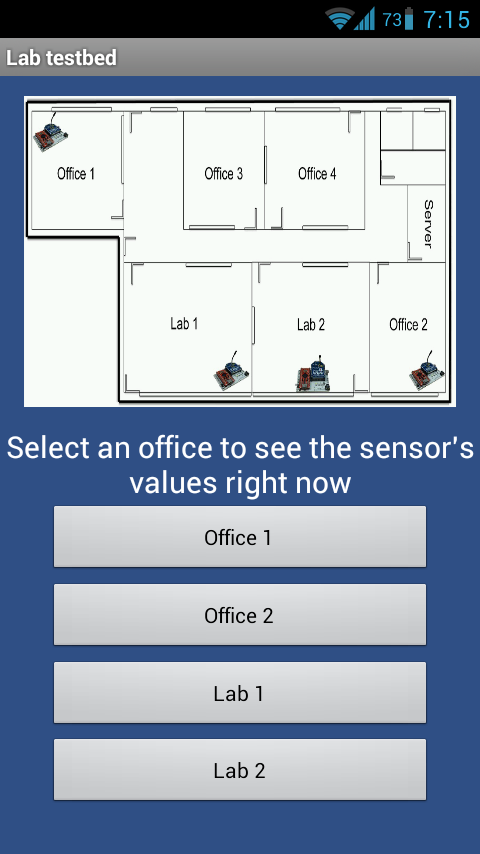
\includegraphics[width=0.5\columnwidth]{images/sensor_topology_screenshot.png}
\label{fig:screen1}}
\hspace{0.2\columnwidth}
\subfigure[Sensor measurement retrieval]{
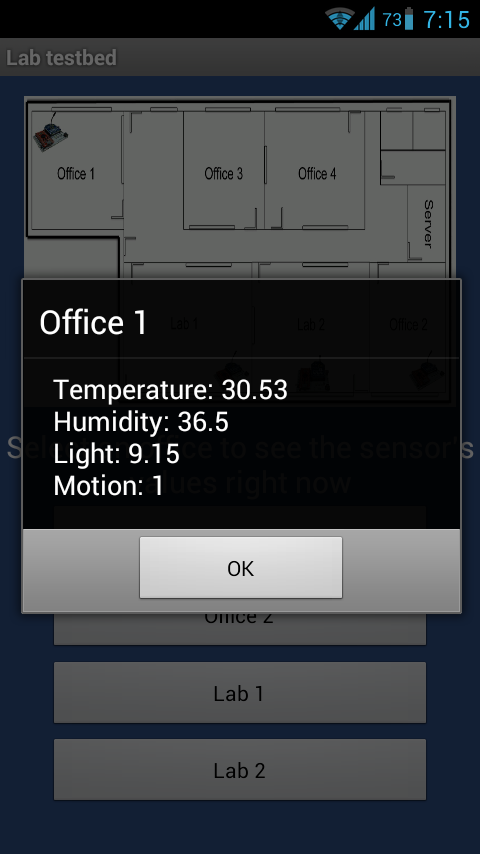
\includegraphics[width=0.5\columnwidth]{images/sensor_data_retrieved_screenshot.png}
\label{fig:screen2}}
\hspace{0.2\columnwidth}
\subfigure[Plugwise manipulation and measurement retrieval]{
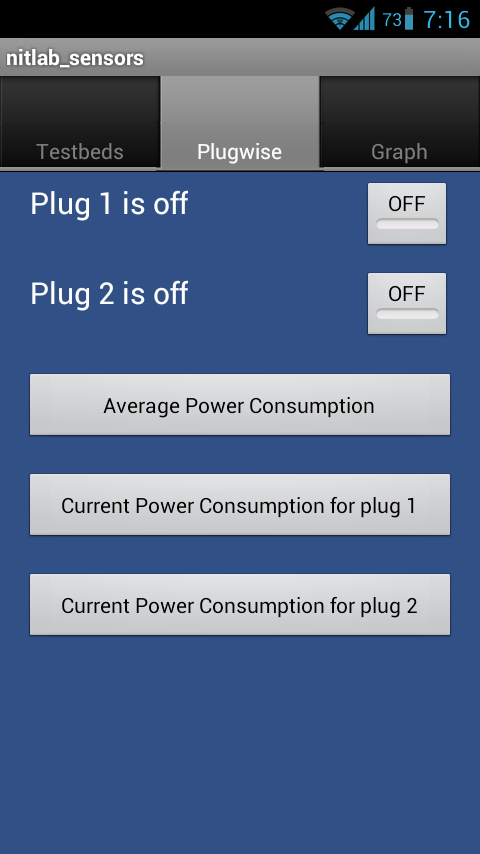
\includegraphics[width=0.5\columnwidth]{images/plugwise_data_screenshot.png}
\label{fig:plugwise_retr}}
\caption{Application Screenshots}
\label{fig:screenshots}

\end{center}
\vspace{-0.8cm}
\end{figure*}




For the demonstration needs, we needed to utilize two different connections to the two servers:
\begin{itemize}
\item A local server was setup, that runs the PlugWise platform software we developed and handles HTTP requests, which exploits the wireless link through the AP to the wireless interface of the Android phone
\item A second remote server that retrieves temperature, humidity, light intensity and human presense measurements from the NITOS wireless sensors. 
\end{itemize}
The second server is using an Internet connection and thus the 3G interface of the Android phone was used for connecting to it. 
A schematic of the overall architecture is depicted in Figure \ref{fig:network}.



% An example of a floating figure using the graphicx package.
% Note that \label must occur AFTER (or within) \caption.
% For figures, \caption should occur after the \includegraphics.
% Note that IEEEtran v1.7 and later has special internal code that
% is designed to preserve the operation of \label within \caption
% even when the captionsoff option is in effect. However, because
% of issues like this, it may be the safest practice to put all your
% \label just after \caption rather than within \caption{}.
%
% Reminder: the "draftcls" or "draftclsnofoot", not "draft", class
% option should be used if it is desired that the figures are to be
% displayed while in draft mode.
%
%\begin{figure}[!t]
%\centering
%\includegraphics[width=2.5in]{myfigure}
% where an .eps filename suffix will be assumed under latex, 
% and a .pdf suffix will be assumed for pdflatex; or what has been declared
% via \DeclareGraphicsExtensions.
%\caption{Simulation Results}
%\label{fig_sim}
%\end{figure}

% Note that IEEE typically puts floats only at the top, even when this
% results in a large percentage of a column being occupied by floats.


% An example of a double column floating figure using two subfigures.
% (The subfig.sty package must be loaded for this to work.)
% The subfigure \label commands are set within each subfloat command, the
% \label for the overall figure must come after \caption.
% \hfil must be used as a separator to get equal spacing.
% The subfigure.sty package works much the same way, except \subfigure is
% used instead of \subfloat.
%
%\begin{figure*}[!t]
%\centerline{\subfloat[Case I]\includegraphics[width=2.5in]{subfigcase1}%
%\label{fig_first_case}}
%\hfil
%\subfloat[Case II]{\includegraphics[width=2.5in]{subfigcase2}%
%\label{fig_second_case}}}
%\caption{Simulation results}
%\label{fig_sim}
%\end{figure*}
%
% Note that often IEEE papers with subfigures do not employ subfigure
% captions (using the optional argument to \subfloat), but instead will
% reference/describe all of them (a), (b), etc., within the main caption.


% An example of a floating table. Note that, for IEEE style tables, the 
% \caption command should come BEFORE the table. Table text will default to
% \footnotesize as IEEE normally uses this smaller font for tables.
% The \label must come after \caption as always.
%
%\begin{table}[!t]
%% increase table row spacing, adjust to taste
%\renewcommand{\arraystretch}{1.3}
% if using array.sty, it might be a good idea to tweak the value of
% \extrarowheight as needed to properly center the text within the cells
%\caption{An Example of a Table}
%\label{table_example}
%\centering
%% Some packages, such as MDW tools, offer better commands for making tables
%% than the plain LaTeX2e tabular which is used here.
%\begin{tabular}{|c||c|}
%\hline
%One & Two\\
%\hline
%Three & Four\\
%\hline
%\end{tabular}
%\end{table}


% Note that IEEE does not put floats in the very first column - or typically
% anywhere on the first page for that matter. Also, in-text middle ("here")
% positioning is not used. Most IEEE journals/conferences use top floats
% exclusively. Note that, LaTeX2e, unlike IEEE journals/conferences, places
% footnotes above bottom floats. This can be corrected via the \fnbelowfloat
% command of the stfloats package.



\section{evaluation}
Our developed application has been developed with the aim to retrieve measurements from the NITOS WSN platform, as well as the remote management of the Plugwise Home Basic Kit.
To this aim, we designed a user friendly GUI, making even the inexperienced users able to operate our platforms.

In Figure \ref{fig:screenshots} we present some indicative screeshots from our application. 
As one can see, the main application window features three separate tabs;
\begin{itemize}
\item 
Testbed
\item 
PlugWise
\item
Graph

\end{itemize}

The first tab refers to the WSN testbed, located at NITLab premises, where the topology of the four wireless sensors are deployed.
As we have mentioned, these four sensors communincate with a dedicated gateway, responsible for collecting and forwarding the sensed measurements.
Using the dedicated buttons for every room, we can retrieve the measurements from the sensors.
The path taken by each request for the sensed data is the following;
When the respective button is pressed, it invokes an HTTP request to the NITLab server. 
The handling function in the backend of our system, issues a request to the sensor gateway for the measurement retrieval.
The sensor gateway broadcasts this request to the dedicated sensors, which push back to it the aggregated data.
The sensor gateway sends this data back to the server, and subsequently back to the phone.
We use a popup window to display the data measured.
The aforementioned described functionality is presented in Figures \ref{fig:screen1} and \ref{fig:screen2} respectively.


\begin{figure*}[!t]
\begin{center}
\centering
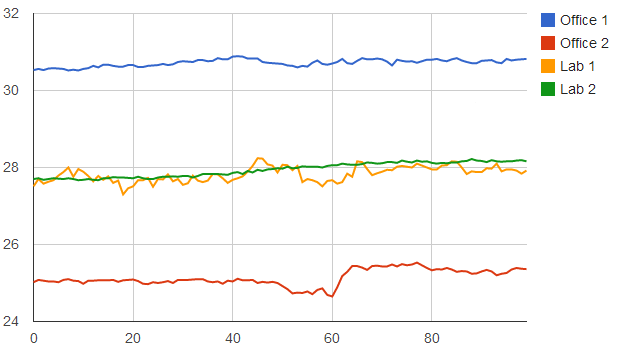
\includegraphics[width=4in]{images/measurements_graph.png}
\caption{Sample line chart presenting data from NITOS WSN}
\label{fig:linechart}
\end{center}
\vspace{-0.8cm}
\end{figure*}



Concerning the plugwise platform manipulation, we use a dedicated tab for it (Figure \ref{fig:plugwise_retr}).
A user can use the interface to interact with the Plugwise "Home Basic Kit", and turn on/off each plug or retrieve information about instantaneous power consumption of each plug, average power consumption of all the plugs and their status.
We utilize a home WLAN connection for this purpose, since in the notion of a SH, all the data generated and aggregated are usually within a single LAN.
An Internet connection could also be utilized for controlling the plugs, however this setup is not so common and requires a server running in the house 24/7.

The data path followed in the case of the Plugwise platform is:
The HTTP request from each button is sent to a local server running in the SH, which handles it and invokes particular scripts on the server responsible for the plugwise platform manipulation.
A key feature of the software developed on the server is a daemon process that retrieves power consumption from the plugs and averages it.
The Plugwise stick is attached to the server, and therefore has full control of the Plugwise Circles.
The data that our server processes produce are then pushed back to the Android application, and presented to the user, using a popup window similar to Figure \ref{fig:screen2}.

Through the Android application, the user can have access to specially created charts, presenting the last measurements from the WSN platform.
The total number of measurements is selected by the user, and presented through a line chart, with different colors from the data sensed by each dedicated sensor.
A sample line chart is presented in Figure \ref{fig:linechart}.

The user has the option of selecting each unique point of the graph, and by a popup window in the Android application, dedicated meassurements are presented back to him/her. 
Each measurement is accompanied with the exact time and date that the specified measurement was taken.



\section{Conclusion}
In this paper we have presented our Android application used to operate and retrieve measurements from SH commercial and experimental sensors.
The overall platform has been evaluated under realistic conditions.


In this age of economic recession, this state-of-the-art technology can provide the opportunity to build an economic business model for application area such as smart homes. 
Building smart homes is a big challenge for worldwide increasing elderly populations which are the largest demographic group of developed countries.


Smart homes obviously have the ability to make life easier and more convenient. They also provide some energy efficiency savings. 
Because wireless systems put some devices at a reduced level of functionality, they can go to "sleep" and wake up when commands are given. 
Some devices can track how much energy each appliance is using and command it to use less. 
Communication between the user and the smart home appliances can be facilitated through the use of extensively used devices such as smart phones using the Android OS. 




% conference papers do not normally have an appendix







% use section* for acknowledgement
\section*{Acknowledgment}


The authors would like to thank the NITLab laboratory for their cooperation, and the fact that they let us use the equipment developed by them. 
We would also like to thank Prof. Thanasis Korakis and Prof. Leandros Tassiulas, directors of the lab, who, with their permission, made this work feasible.


%\cite{pursuit}

% trigger a \newpage just before the given reference
% number - used to balance the columns on the last page
% adjust value as needed - may need to be readjusted if
% the document is modified later
%\IEEEtriggeratref{8}
% The "triggered" command can be changed if desired:
%\IEEEtriggercmd{\enlargethispage{-5in}}


%\bibliography{eam}
%\bibliographystyle{unsrt}

\begin{thebibliography}{9}

\bibitem{howshswork}
 How Smart Homes Work, \url{http://home.howstuffworks.com/smart-home.htm/}.

\bibitem{paper}
 Design and implementation of wireless Smart-home sensor network based on ZigBee protocol, Lili Liang and Lianfen Huang and Xueyuan Jiang and Yan Yao, In the proceedings of ICCCAS 2008.

\bibitem{wikiwsn}
Wireless Sensor Network, \url{http://en.wikipedia.org/wiki/Wireless_sensor_network/}.

\bibitem{howwifiworks}
How WiFi Works, \url{http://computer.howstuffworks.com/wireless-network.htm/}.

\bibitem{zigbee}
ZigBee protocol, \url{http://en.wikipedia.org/wiki/ZigBee/}.

\bibitem{android}
Android Operating System, \url{https://en.wikipedia.org/wiki/Android_(operating_system)}.

\bibitem{nitlab}
Network Implementation Testbed Laboratory, \url{http://nitlab.inf.uth.gr/NITlab/}.

\bibitem{promicro}
Pro Micro Board, \url{https://www.sparkfun.com/products/10999/}.

\bibitem{sparkfun}
Sparkfun Electronics, \url{https://www.sparkfun.com/}.

\bibitem{arduino}
Arduino, \url{http://www.arduino.cc/}.

\bibitem{arduino-ide}
Arduino-IDE, \url{http://arduino.cc/en/Main/Software/}.

\bibitem{atmel}
Atmel Corporation, \url{http://www.atmel.com/}.

\bibitem{xbee}
Xbee radio interfaces, \url{http://www.digi.com/xbee/}.

\bibitem{zigbee-all}
ZigBee Alliance, \url{http://www.zigbee.org/}.

\bibitem{plugwise}
Plugwise Source, \url{http://www.plugwise.com/idplugtype-f/source}.

\end{thebibliography}






% that's all folks
\end{document}


